\documentclass[11pt,a4paper]{article}

% ---------- arXiv-safe packages (pdfLaTeX, standard TeX Live only) ----------
\usepackage[utf8]{inputenc}
\usepackage[T1]{fontenc}
\usepackage{lmodern}
\usepackage[margin=1in]{geometry}
\usepackage{amsmath,amssymb,bm}
\usepackage{booktabs,tabularx,array}
\usepackage{graphicx}
\usepackage{xcolor}
\usepackage{caption}
\usepackage{microtype}
\usepackage{setspace}
\usepackage[authoryear,round]{natbib}
\usepackage{listings}
\usepackage{pgfplots}
\usepgfplotslibrary{groupplots}
\pgfplotsset{compat=1.16}
\usepackage[colorlinks=true,linkcolor=blue!50!black,citecolor=blue!50!black,urlcolor=blue!50!black]{hyperref}

\onehalfspacing
\emergencystretch=2em
\setlength{\parindent}{1.5em}
\setlength{\parskip}{0pt}
\captionsetup{font=small,labelfont=bf}

% ---------- code listings ----------
\lstdefinestyle{py}{
  language=Python,
  basicstyle=\ttfamily\scriptsize,
  keywordstyle=\bfseries\color{blue!55!black},
  commentstyle=\itshape\color{green!40!black},
  stringstyle=\color{red!50!black},
  numbers=left, numberstyle=\tiny\color{gray}, numbersep=6pt,
  frame=single, rulecolor=\color{gray!60},
  breaklines=true, breakatwhitespace=false,
  columns=fullflexible, keepspaces=true,
  showstringspaces=false, tabsize=4,
  captionpos=t, aboveskip=1em, belowskip=0.5em
}
\lstset{style=py}

\newcommand{\simnote}{simulated data, pipeline validation only}

\title{Decomposing the Contribution of Artificial Intelligence to Macroeconomic Productivity:\\
A Growth Accounting and Panel Regression Approach}
\author{First Author\thanks{Affiliation, e-mail.} \and Second Author\thanks{Affiliation, e-mail.}}
\date{\today}

\begin{document}
\maketitle

\begin{abstract}
Output growth that coincides with the spread of artificial intelligence (AI) cannot be treated as an AI-driven productivity gain, because capital accumulation, labour growth and changes in workforce quality also raise output. This paper sets out a two-stage design that separates these sources. The first stage estimates a log-linear Cobb--Douglas production function by ordinary least squares with country, sector and year fixed effects and uses the estimated elasticities to decompose output growth into capital, labour and total factor productivity (TFP) contributions. The second stage regresses TFP growth on an AI adoption measure, with controls, fixed effects and country-clustered standard errors, in current and lagged specifications. The design is implemented in a reproducible Python pipeline using World Bank and OECD data. The numerical results reported here come from a simulated panel with known parameters and validate the estimators only. They carry no information about the real economy.
\end{abstract}

\noindent\textbf{Keywords:} artificial intelligence; total factor productivity; growth accounting; Cobb--Douglas production function; panel data; fixed effects\\
\textbf{JEL codes:} O33, O47, C23, E23

% =====================================================================
\section{Introduction}
Measuring the effect of artificial intelligence on productivity is considerably more difficult than observing its spread across an economy. An increase in output following the adoption of AI cannot automatically be treated as an AI driven productivity gain, since output may also rise because of capital accumulation, growth in labour input, improvements in workforce quality or broader changes in economic conditions. The problem is further complicated by the way AI investment appears in economic statistics. Expenditure on hardware and some forms of software may be recorded as capital formation, while investments in data, organisational restructuring and technical knowledge may be measured incompletely or omitted altogether. Consequently, the recorded contribution of AI may differ from its underlying economic contribution. \citet{corrado2021} show that conventional productivity measures can overlook parts of AI investment because the technology combines measured tangible assets with less visible intangible assets. \citet{brynjolfsson2017} similarly describe a modern productivity paradox in which rapid technological progress does not immediately appear in aggregate productivity statistics. The central challenge is therefore not simply to determine whether productivity and AI adoption move together, but to separate the contribution associated with AI from the other forces shaping output at the same time.

This measurement problem becomes particularly significant at the macroeconomic level. Artificial intelligence may require complementary investment in infrastructure, data, human capital and institutional capacity before its effects become visible in recorded output. \citet{brynjolfsson2021} demonstrate that these complementary investments can initially suppress measured productivity growth before their benefits emerge, creating what they describe as a productivity J curve. The scale and timing of any productivity effect may also vary according to the structure of an economy. Recent OECD estimates indicate that expected productivity gains from AI differ across countries because exposure, adoption and sectoral composition are not uniform \citep{filippucci2024}. This means that a single correlation between AI adoption and output growth may conceal substantial differences in the conditions under which the technology is introduced. It may also incorrectly attribute to AI changes that are actually generated by capital expansion or labour growth. A credible macroeconomic assessment must therefore distinguish between growth arising from additional productive inputs and growth arising from a more efficient use of those inputs.

This study addresses that problem through a three factor growth decomposition model followed by panel regression analysis. Growth accounting, developed by \citet{solow1957} and refined by \citet{jorgenson1967}, remains the conventional benchmark for separating output growth into the contributions of capital, labour and total factor productivity. The model first calculates how much of the observed change in output can be explained by changes in capital and labour. The remaining component is recorded as total factor productivity, which captures changes in the efficiency with which those inputs are combined. An AI adoption measure is then introduced into a fixed effects OLS regression to examine whether changes in AI adoption are systematically associated with the productivity component after observable economic influences and persistent differences between countries and sectors have been taken into account. This approach does not assume that every increase in output occurring alongside AI adoption was caused by AI. Instead, it begins with the established sources of economic growth and tests whether AI provides additional explanatory power once those sources have been separated. In doing so, the study places the analysis of artificial intelligence within a recognised macroeconomic framework while responding to the measurement difficulties identified in the existing literature.

% =====================================================================
\section{Methodology}
This study uses a quantitative macroeconomic design combining growth accounting with panel data regression. The unit of observation is a country, sector and year. The principal variables are real sectoral output, capital input, labour input and an indicator of artificial intelligence adoption or exposure. Output and input data will be drawn from the World Bank and expressed in constant prices wherever monetary values are used. The panel structure allows the study to examine changes both across economies and over time while controlling for characteristics that are not directly observable but remain relatively stable within a country or sector.

The first stage applies the three factor growth decomposition associated with the Solow growth accounting framework. This method has been used extensively in productivity research since \citet{solow1957}, while \citet{jorgenson1967} developed a more detailed treatment of how changes in productive inputs should be measured. Related research on artificial intelligence has continued to use productivity accounting frameworks to examine how tangible and intangible technological investment enters measured output and total factor productivity \citep{corrado2021}. The method begins with a constant returns Cobb--Douglas production function:
\begin{equation}
  Y_{cst} = A_{cst}\,K_{cst}^{\alpha}\,L_{cst}^{\beta},
  \label{eq:cd}
\end{equation}
where $Y_{cst}$ represents real output in country $c$, sector $s$ and year $t$, $K_{cst}$ is the capital input, $L_{cst}$ is the labour input and $A_{cst}$ represents total factor productivity. The coefficients $\alpha$ and $\beta$ measure the output elasticities of capital and labour. Under the constant returns assumption:
\begin{equation}
  \alpha + \beta = 1.
  \label{eq:crs}
\end{equation}
Taking natural logarithms gives:
\begin{equation}
  \ln Y_{cst} = \ln A_{cst} + \alpha \ln K_{cst} + \beta \ln L_{cst}.
\end{equation}
The production function will initially be estimated through OLS with country, sector and year fixed effects:
\begin{equation}
  \ln Y_{cst} = a + \alpha \ln K_{cst} + \beta \ln L_{cst} + \mu_c + \eta_s + \tau_t + u_{cst}.
  \label{eq:pf}
\end{equation}
In this equation, $a$ is the constant term, $\mu_c$ represents country fixed effects, $\eta_s$ represents sector fixed effects, $\tau_t$ represents year fixed effects and $u_{cst}$ is the error term. Country fixed effects account for persistent national differences such as geography, institutions and long established infrastructure. Sector fixed effects account for structural differences between areas of production, while year fixed effects absorb shocks shared across the sample, including global economic disruptions and common technological changes.

After estimating the capital and labour coefficients, annual output growth is decomposed into three parts:
\begin{equation}
  \Delta \ln Y_{cst} = \hat{\alpha}\,\Delta \ln K_{cst} + \hat{\beta}\,\Delta \ln L_{cst} + \Delta \ln A_{cst}.
\end{equation}
The first component is the contribution of capital growth. The second is the contribution of labour growth. The third is total factor productivity growth. TFP growth is calculated as the residual:
\begin{equation}
  \Delta \ln A_{cst} = \Delta \ln Y_{cst} - \hat{\alpha}\,\Delta \ln K_{cst} - \hat{\beta}\,\Delta \ln L_{cst}.
\end{equation}
For calculation purposes, the logarithmic growth rate of any variable $X$ is:
\begin{equation}
  g_X = 100\,(\ln X_t - \ln X_{t-1}).
\end{equation}
The three contributions are therefore calculated as:
\begin{align}
  C_K &= \hat{\alpha}\, g_K, \\
  C_L &= \hat{\beta}\, g_L, \\
  C_{TFP} &= g_Y - C_K - C_L.
\end{align}
Suppose, for example, that real output grows by 5 per cent, capital grows by 6 per cent and labour grows by 2 per cent. If the estimated capital elasticity is 0.40, the labour elasticity under constant returns is 0.60. The capital contribution would equal $0.40 \times 6 = 2.4$ percentage points, while the labour contribution would equal $0.60 \times 2 = 1.2$ percentage points. TFP growth would then be:
\begin{equation}
  5 - 2.4 - 1.2 = 1.4.
\end{equation}
The calculation would therefore attribute 2.4 percentage points of output growth to capital, 1.2 percentage points to labour and the remaining 1.4 percentage points to improved total factor productivity.

The second stage investigates whether AI adoption helps explain the calculated change in TFP. The main specification is a fixed effects OLS regression:
\begin{equation}
  \Delta \ln A_{cst} = \delta + \theta\, AI_{cst} + \bm{\gamma}'\mathbf{X}_{cst} + \mu_c + \eta_s + \tau_t + \varepsilon_{cst}.
  \label{eq:stage2}
\end{equation}
Here, $\Delta \ln A_{cst}$ is the estimated rate of TFP growth, $AI_{cst}$ is the measure of AI adoption or exposure, and $\mathbf{X}_{cst}$ is a vector of control variables. These controls may include education, research expenditure, digital infrastructure, trade openness and the level of economic development, subject to data availability. The coefficient $\theta$ is the main coefficient of interest. It measures the estimated change in TFP growth associated with a one unit increase in the AI variable after the control variables and fixed effects have been considered.

The regression coefficients are obtained by minimising the sum of squared residuals. In matrix form, the OLS estimator is:
\begin{equation}
  \hat{\bm{b}} = (\mathbf{X}'\mathbf{X})^{-1}\mathbf{X}'\mathbf{y},
  \label{eq:ols}
\end{equation}
where $\mathbf{y}$ contains the observations of TFP growth and $\mathbf{X}$ contains the AI indicator, control variables and fixed effect terms. Because observations from the same country may remain correlated across years, standard errors will be clustered at the country level. A lagged specification will also be estimated because the productivity effects of AI may take time to appear:
\begin{equation}
  \Delta \ln A_{cst} = \delta + \theta\, AI_{cs,t-1} + \bm{\gamma}'\mathbf{X}_{cst} + \mu_c + \eta_s + \tau_t + \varepsilon_{cst}.
  \label{eq:stage2lag}
\end{equation}
This additional model reflects previous research showing that new technologies may require complementary investment and organisational adjustment before their effects become visible in productivity statistics \citep{brynjolfsson2021}. The current and lagged specifications will be compared to determine whether the relationship appears immediately or with a delay. The estimated contribution associated with a change in AI adoption can subsequently be calculated as:
\begin{equation}
  C_{AI} = \hat{\theta}\,(AI_{cst} - AI_{cs,t-1}).
\end{equation}

The decomposition and regression perform different but complementary roles. The decomposition prevents capital and labour growth from being mistaken for productivity improvement. The regression then tests whether AI adoption is associated with the remaining productivity component after common shocks, persistent country and sector differences and observable control variables have been considered. The coefficient should be interpreted as a conditional association unless the study introduces an additional identification strategy, such as a valid instrumental variable or a clearly defined policy shock. The model therefore provides a disciplined estimate of the relationship between AI and macroeconomic productivity without claiming causation beyond what the data and research design can support.

% =====================================================================
\section{The Cobb--Douglas Production Function: Diagram and Log-Linear OLS Estimation}
\subsection{Explaining the diagram}
Figure~\ref{fig:cd} plots the production function $Y = AK^{\alpha}L^{\beta}$ with $A=1$, $\alpha=0.4$ and $\beta=0.6$ in three complementary views.

\begin{figure}[t]
\centering
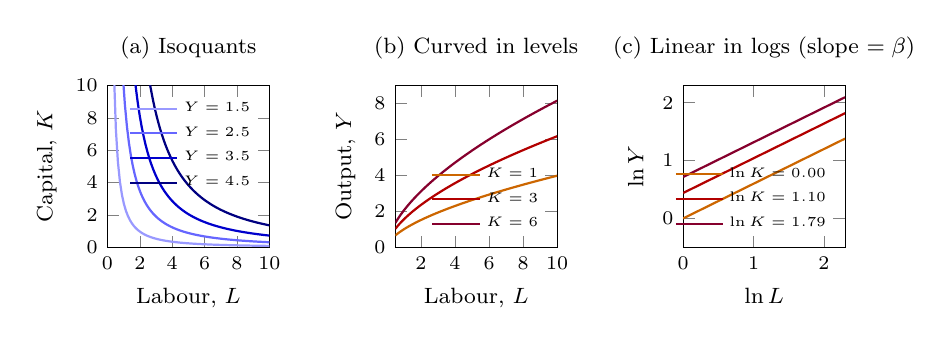
\begin{tikzpicture}
\begin{groupplot}[
  group style={group size=3 by 1, horizontal sep=1.6cm},
  width=0.3\textwidth, height=0.3\textwidth,
  tick label style={font=\scriptsize}, label style={font=\footnotesize},
  title style={font=\footnotesize}, legend style={font=\tiny, draw=none, fill=none},
  legend cell align=left]
\nextgroupplot[title={(a) Isoquants}, xlabel={Labour, $L$}, ylabel={Capital, $K$},
  xmin=0, xmax=10, ymin=0, ymax=10, legend pos=north east]
  \addplot[blue!40!white, thick, domain=0.15:10, samples=80] {(1.5/(x^0.6))^(1/0.4)};
  \addplot[blue!60!white, thick, domain=0.35:10, samples=80] {(2.5/(x^0.6))^(1/0.4)};
  \addplot[blue!80!black, thick, domain=0.7:10, samples=80] {(3.5/(x^0.6))^(1/0.4)};
  \addplot[blue!50!black, thick, domain=1.1:10, samples=80] {(4.5/(x^0.6))^(1/0.4)};
  \legend{$Y=1.5$,$Y=2.5$,$Y=3.5$,$Y=4.5$}
\nextgroupplot[title={(b) Curved in levels}, xlabel={Labour, $L$}, ylabel={Output, $Y$},
  xmin=0.5, xmax=10, ymin=0, ymax=9, legend pos=south east]
  \addplot[orange!80!black, thick, domain=0.5:10, samples=60] {1^0.4*x^0.6};
  \addplot[red!70!black, thick, domain=0.5:10, samples=60] {3^0.4*x^0.6};
  \addplot[purple!70!black, thick, domain=0.5:10, samples=60] {6^0.4*x^0.6};
  \legend{$K=1$,$K=3$,$K=6$}
\nextgroupplot[title={(c) Linear in logs (slope $=\beta$)}, xlabel={$\ln L$}, ylabel={$\ln Y$},
  xmin=0, xmax=2.3, ymin=-0.5, ymax=2.3, legend pos=south east]
  \addplot[orange!80!black, thick, domain=0:2.3] {0.4*0 + 0.6*x};
  \addplot[red!70!black, thick, domain=0:2.3] {0.4*1.10 + 0.6*x};
  \addplot[purple!70!black, thick, domain=0:2.3] {0.4*1.79 + 0.6*x};
  \legend{$\ln K=0.00$,$\ln K=1.10$,$\ln K=1.79$}
\end{groupplot}
\end{tikzpicture}
\caption{The Cobb--Douglas production function ($A=1$, $\alpha=0.4$, $\beta=0.6$): (a) isoquants, (b) output against labour for fixed capital, (c) the same relationship after taking logarithms.}
\label{fig:cd}
\end{figure}

\paragraph{Panel (a), isoquants.} Each curve joins all combinations of capital and labour that yield the same output. Curves further from the origin represent higher output. They slope downward because the two inputs are substitutes: if less labour is used, more capital is needed to hold output constant. They are convex to the origin because substitution becomes progressively harder as one input becomes scarce. The slope of an isoquant is the marginal rate of technical substitution, $\mathrm{MRTS} = MP_L/MP_K = (\beta/\alpha)(K/L)$.

\paragraph{Panel (b), diminishing returns.} Holding capital fixed, output rises with labour at a decreasing rate because $\beta<1$. The marginal product of labour is $MP_L = \beta Y/L$, which falls as $L$ grows. A larger capital stock shifts the whole curve upward, showing that capital and labour are complements. A change in total factor productivity $A$ would also scale every curve upward in the same proportion.

\paragraph{Panel (c), the log transformation.} Once both axes are logged, each curve becomes a straight line with slope $\beta$ and intercept $\ln A + \alpha\ln K$. Changing capital moves the line up or down in parallel without changing its slope. This is the property that makes the production function estimable by ordinary least squares.

\subsection{From a non-linear function to a linear regression}
OLS requires a model that is linear in its parameters. The Cobb--Douglas function is not, because $\alpha$ and $\beta$ enter as exponents. Introducing a multiplicative error term and taking natural logarithms resolves this:
\begin{equation}
  Y_{cst} = A_{cst}K_{cst}^{\alpha}L_{cst}^{\beta}e^{u_{cst}}
  \;\Longrightarrow\;
  \ln Y_{cst} = \ln A_{cst} + \alpha\ln K_{cst} + \beta\ln L_{cst} + u_{cst}.
\end{equation}
The right-hand side is now a linear combination of the unknown coefficients $\alpha$ and $\beta$, so the estimator in Section~2 applies directly. With $\mathbf{y}$ the vector of $\ln Y_{cst}$ and $\mathbf{X}$ the matrix containing a constant, $\ln K_{cst}$, $\ln L_{cst}$ and the country, sector and year dummies, OLS chooses the coefficients that minimise $\sum u_{cst}^2$, giving $\hat{\bm{b}} = (\mathbf{X}'\mathbf{X})^{-1}\mathbf{X}'\mathbf{y}$. The persistent part of $\ln A_{cst}$ is captured by the fixed effects, and the remainder is left in the residual, which is what the growth decomposition later treats as TFP.

The logarithmic form also gives the coefficients a direct economic meaning. Since $\alpha = \partial\ln Y/\partial\ln K$, it is the elasticity of output with respect to capital: a 10 per cent increase in capital raises output by $10\alpha$ per cent. With $\alpha=0.4$ this is 4 per cent, which matches the worked example in Section~2.

Under constant returns to scale ($\alpha+\beta=1$) the regression can be written in per-worker form:
\begin{equation}
  \ln\!\left(\frac{Y_{cst}}{L_{cst}}\right) = a + \alpha\ln\!\left(\frac{K_{cst}}{L_{cst}}\right) + \mu_c + \eta_s + \tau_t + u_{cst},
  \qquad \beta = 1-\hat{\alpha}.
\end{equation}
This has a single regressor and imposes the restriction directly. The study estimates both forms, tests $\alpha+\beta=1$ with a $t$-test on the unrestricted model, and uses the restricted $\hat{\alpha}$ in the decomposition. Two caveats apply. First, the log transformation requires strictly positive output and inputs. Second, OLS gives consistent elasticities only if the inputs are uncorrelated with the error term. Firms that expect high productivity may invest and hire more, so the estimates should be read as conditional associations, as stated in Section~2.

% =====================================================================
\section{Results and Analysis}
\subsection{Data and implementation}
The analysis is implemented in Python (the listings below) and pulls data directly from the REST APIs of the World Bank and the OECD. Table~\ref{tab:data} lists what is used.

\begin{table}[t]
\centering
\small
\begin{tabularx}{\textwidth}{@{}l>{\raggedright\arraybackslash}X>{\raggedright\arraybackslash}X@{}}
\toprule
Variable & Source and series & Construction \\
\midrule
Output $Y$ & World Bank value added by sector (agriculture, industry, services), constant 2015 US\$ & Used as is \\
Labour $L$ & World Bank labour force, unemployment rate and sectoral employment shares & Employment $\times$ sector share \\
Capital $K$ & World Bank gross fixed capital formation, constant 2015 US\$ & Perpetual inventory, $\delta=5\%$, allocated to sectors by employment share \\
AI adoption & OECD ICT Access and Usage by Businesses (\texttt{DSD\_ICT\_B@DF\_BUSINESSES}), enterprises using AI & Country-year, 2021 onward where available \\
Controls $\mathbf{X}$ & World Bank GDP per capita, tertiary enrolment, R\&D spending, trade openness, internet users & Used where coverage is adequate \\
\bottomrule
\end{tabularx}
\caption{Data sources and construction.}
\label{tab:data}
\end{table}

Three limitations should be kept in mind. The World Bank does not publish sectoral capital stocks, so country capital is allocated to sectors in proportion to employment. This makes sectoral capital per worker identical across sectors within a country and year, and it means the capital elasticity is identified from country-level capital deepening. Replacing this step with sectoral capital from OECD STAN or EU KLEMS would improve the design. The OECD AI indicator is only available for recent years and for a limited set of countries, so the second-stage panel is short. The AI measure is also recorded at the country level and is therefore repeated across sectors. Standard errors are clustered by country, which partly accounts for this.

\subsection{Python code}
The code is split into seven blocks, each in its own module, and executed in order by \texttt{run\_analysis.py}. Downloads are cached in a \texttt{cache} folder, so each API is called only once. Running \texttt{python run\_analysis.py} downloads the data, estimates both stages and writes the tables, figures and a text log (\texttt{run\_log.txt}) to the \texttt{results} folder. The source files accompany this paper in the \texttt{code/} directory.

\lstinputlisting[caption={Block 0: settings (\texttt{config.py})},label={lst:config}]{code/config.py}
\lstinputlisting[caption={Block 0: cached downloads and run log (\texttt{utils.py})},label={lst:utils}]{code/utils.py}
\lstinputlisting[caption={Block 1: World Bank REST API (\texttt{api\_worldbank.py})},label={lst:wb}]{code/api_worldbank.py}
\lstinputlisting[caption={Block 2: OECD SDMX REST API (\texttt{api\_oecd.py})},label={lst:oecd}]{code/api_oecd.py}
\lstinputlisting[caption={Block 3: building the panel (\texttt{panel.py})},label={lst:panel}]{code/panel.py}
\lstinputlisting[caption={Block 4: log-linear OLS and growth accounting (\texttt{stage1.py})},label={lst:stage1}]{code/stage1.py}
\lstinputlisting[caption={Block 5: AI and TFP regressions (\texttt{stage2.py})},label={lst:stage2}]{code/stage2.py}
\lstinputlisting[caption={Block 6: tables and figures (\texttt{reporting.py})},label={lst:report}]{code/reporting.py}
\lstinputlisting[caption={Runner that executes the blocks in order (\texttt{run\_analysis.py})},label={lst:run}]{code/run_analysis.py}

\subsection{Output}
\textbf{The numbers in this subsection come from simulated data and serve pipeline validation only.} They were generated on a simulated panel of 60 countries and three sectors with known parameters ($\alpha=0.40$, AI effect $\theta=0.10$) because the environment used to prepare this draft cannot reach the World Bank and OECD domains. They show that the estimators work as intended and nothing about the real economy. Running the code on a machine with internet access replaces them with results from the live APIs.

\begin{table}[t]
\centering
\begin{tabular}{lrr}
\toprule
 & Estimate & Std.\ error \\
\midrule
$\alpha$ (unrestricted) & 0.416 & 0.004 \\
$\beta$ (unrestricted) & 0.611 & 0.004 \\
$\alpha+\beta$ (unrestricted) & 1.027 & 0.006 \\
$\alpha$ (CRS imposed) & 0.404 & 0.003 \\
$\beta=1-\alpha$ (CRS imposed) & 0.596 & 0.003 \\
\bottomrule
\end{tabular}
\caption{Stage 1: production function estimates with country, sector and year fixed effects and country-clustered standard errors (\simnote).}
\label{tab:pf}
\end{table}

\begin{table}[t]
\centering
\begin{tabular}{lrrrr}
\toprule
 & Output growth & Capital & Labour & TFP \\
\midrule
Agriculture & 4.08 & 1.66 & 0.64 & 1.78 \\
Industry    & 3.97 & 1.61 & 0.59 & 1.78 \\
Services    & 3.92 & 1.62 & 0.60 & 1.71 \\
\bottomrule
\end{tabular}
\caption{Mean annual growth decomposition, percentage points (\simnote).}
\label{tab:dec}
\end{table}

\begin{figure}[t]
\centering
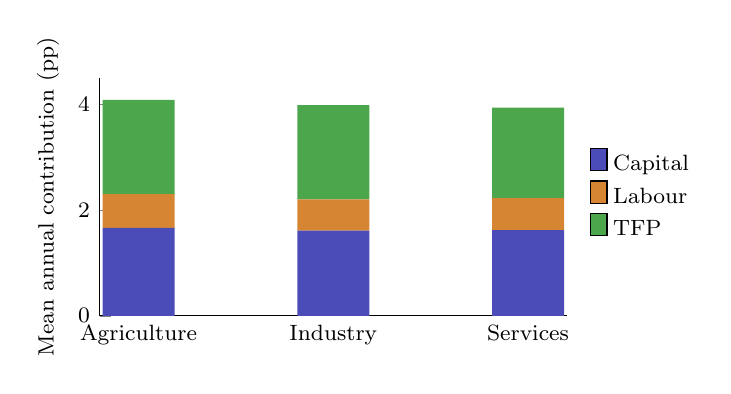
\begin{tikzpicture}
\begin{axis}[
  ybar stacked, bar width=26pt, width=0.62\textwidth, height=0.38\textwidth,
  symbolic x coords={Agriculture,Industry,Services}, xtick=data,
  ymin=0, ymax=4.5, ylabel={Mean annual contribution (pp)},
  tick label style={font=\footnotesize}, label style={font=\footnotesize},
  legend style={font=\footnotesize, at={(1.03,0.5)}, anchor=west, draw=none},
  legend cell align=left, axis x line*=bottom, axis y line*=left]
\addplot[fill=blue!60!black!70, draw=none] coordinates {(Agriculture,1.66) (Industry,1.61) (Services,1.62)};
\addplot[fill=orange!80!black!80, draw=none] coordinates {(Agriculture,0.64) (Industry,0.59) (Services,0.60)};
\addplot[fill=green!50!black!70, draw=none] coordinates {(Agriculture,1.78) (Industry,1.78) (Services,1.71)};
\legend{Capital,Labour,TFP}
\end{axis}
\end{tikzpicture}
\caption{Contribution of capital, labour and TFP to output growth by sector (\simnote).}
\label{fig:dec}
\end{figure}

\begin{table}[t]
\centering
\begin{tabular}{lrrrrrr}
\toprule
 & $\theta$ & Std.\ error & $p$-value & $N$ & Countries & $R^2$ \\
\midrule
Current AI & 0.093 & 0.017 & 0.000 & 2520 & 60 & 0.164 \\
Lagged AI  & 0.095 & 0.017 & 0.000 & 2340 & 60 & 0.155 \\
\bottomrule
\end{tabular}
\caption{Stage 2: effect of AI adoption on TFP growth (percentage points per unit of AI), current and lagged specifications (\simnote).}
\label{tab:ai}
\end{table}

\subsection{Analysis}
\paragraph{Production function.} The unrestricted estimates in Table~\ref{tab:pf} sum to a value close to one, and the constant-returns estimate of $\alpha$ is close to the true value of 0.40. This shows that the log-linear OLS step recovers the capital elasticity correctly when the data follow a Cobb--Douglas process. With real data the same table reports the elasticities that feed the decomposition, together with the test of constant returns.

\paragraph{Decomposition.} In Table~\ref{tab:dec} the contributions of capital and labour are the estimated elasticities multiplied by the growth rates of each input, and TFP is what remains. Capital accumulation accounts for a large share of output growth in this simulation, so an observer who attributed all growth to efficiency would overstate the role of productivity. With real data this table shows which sectors grow through accumulation and which through efficiency gains.

\paragraph{AI and TFP growth.} Table~\ref{tab:ai} reports $\hat\theta$, the change in TFP growth associated with a one-unit increase in AI adoption. In the validation run both specifications give estimates close to the true value of 0.10. The contribution of a given change in adoption follows from $C_{AI} = \hat\theta(AI_{cst} - AI_{cs,t-1})$. Comparing the current and lagged rows indicates whether any effect appears immediately or with a delay, in line with the productivity J-curve argument of \citet{brynjolfsson2021}.

\paragraph{Interpretation with real data.} A statistically significant $\hat\theta$ would show that, after fixed effects and controls, higher AI adoption is associated with faster TFP growth. A small or insignificant value would be consistent with a delayed effect, with mismeasured AI investment, or with a sample that is too short, and should not be read as proof that AI has no effect. As stated in the methodology, $\hat\theta$ is a conditional association rather than a causal effect unless an instrument or policy shock is added.

% =====================================================================
\begin{thebibliography}{6}
\setlength{\itemsep}{2pt}

\bibitem[Brynjolfsson et~al.(2017)]{brynjolfsson2017}
Brynjolfsson, E., Rock, D., and Syverson, C. (2017).
\newblock Artificial intelligence and the modern productivity paradox: A clash of expectations and statistics.
\newblock NBER Working Paper No.\ 24001, National Bureau of Economic Research.

\bibitem[Brynjolfsson et~al.(2021)]{brynjolfsson2021}
Brynjolfsson, E., Rock, D., and Syverson, C. (2021).
\newblock The productivity J-curve: How intangibles complement general purpose technologies.
\newblock \emph{American Economic Journal: Macroeconomics}, 13(1):333--372.

\bibitem[Corrado et~al.(2021)]{corrado2021}
Corrado, C., Haskel, J., and Jona-Lasinio, C. (2021).
\newblock Artificial intelligence and productivity: an intangible assets approach.
\newblock \emph{Oxford Review of Economic Policy}, 37(3):435--458.

\bibitem[Filippucci et~al.(2024)]{filippucci2024}
Filippucci, F., Gal, P., Jona-Lasinio, C., Leandro, A., and Nicoletti, G. (2024).
\newblock The impact of artificial intelligence on productivity, distribution and growth: Key mechanisms, initial evidence and policy challenges.
\newblock OECD Artificial Intelligence Papers No.\ 15, OECD Publishing, Paris.

\bibitem[Jorgenson and Griliches(1967)]{jorgenson1967}
Jorgenson, D.~W. and Griliches, Z. (1967).
\newblock The explanation of productivity change.
\newblock \emph{Review of Economic Studies}, 34(3):249--283.

\bibitem[Solow(1957)]{solow1957}
Solow, R.~M. (1957).
\newblock Technical change and the aggregate production function.
\newblock \emph{Review of Economics and Statistics}, 39(3):312--320.

\end{thebibliography}

\end{document}
